% Options for packages loaded elsewhere
\PassOptionsToPackage{unicode}{hyperref}
\PassOptionsToPackage{hyphens}{url}
\PassOptionsToPackage{dvipsnames,svgnames,x11names}{xcolor}
%
\documentclass[
  ignorenonframetext,
]{beamer}
\usepackage{pgfpages}
\setbeamertemplate{caption}[numbered]
\setbeamertemplate{caption label separator}{: }
\setbeamercolor{caption name}{fg=normal text.fg}
\beamertemplatenavigationsymbolsempty
% Prevent slide breaks in the middle of a paragraph
\widowpenalties 1 10000
\raggedbottom

\usepackage{amsmath,amssymb}
\usepackage{iftex}
\ifPDFTeX
  \usepackage[T1]{fontenc}
  \usepackage[utf8]{inputenc}
  \usepackage{textcomp} % provide euro and other symbols
\else % if luatex or xetex
  \usepackage{unicode-math}
  \defaultfontfeatures{Scale=MatchLowercase}
  \defaultfontfeatures[\rmfamily]{Ligatures=TeX,Scale=1}
\fi
\usepackage{lmodern}
\usetheme[]{AnnArbor}
\usecolortheme{dolphin}
\usefonttheme{structurebold}
\ifPDFTeX\else  
    % xetex/luatex font selection
\fi
% Use upquote if available, for straight quotes in verbatim environments
\IfFileExists{upquote.sty}{\usepackage{upquote}}{}
\IfFileExists{microtype.sty}{% use microtype if available
  \usepackage[]{microtype}
  \UseMicrotypeSet[protrusion]{basicmath} % disable protrusion for tt fonts
}{}
\makeatletter
\@ifundefined{KOMAClassName}{% if non-KOMA class
  \IfFileExists{parskip.sty}{%
    \usepackage{parskip}
  }{% else
    \setlength{\parindent}{0pt}
    \setlength{\parskip}{6pt plus 2pt minus 1pt}}
}{% if KOMA class
  \KOMAoptions{parskip=half}}
\makeatother
\usepackage{xcolor}
\newif\ifbibliography
\setlength{\emergencystretch}{3em} % prevent overfull lines
\setcounter{secnumdepth}{-\maxdimen} % remove section numbering


\providecommand{\tightlist}{%
  \setlength{\itemsep}{0pt}\setlength{\parskip}{0pt}}\usepackage{longtable,booktabs,array}
\usepackage{calc} % for calculating minipage widths
\usepackage{caption}
% Make caption package work with longtable
\makeatletter
\def\fnum@table{\tablename~\thetable}
\makeatother
\usepackage{graphicx}
\makeatletter
\def\maxwidth{\ifdim\Gin@nat@width>\linewidth\linewidth\else\Gin@nat@width\fi}
\def\maxheight{\ifdim\Gin@nat@height>\textheight\textheight\else\Gin@nat@height\fi}
\makeatother
% Scale images if necessary, so that they will not overflow the page
% margins by default, and it is still possible to overwrite the defaults
% using explicit options in \includegraphics[width, height, ...]{}
\setkeys{Gin}{width=\maxwidth,height=\maxheight,keepaspectratio}
% Set default figure placement to htbp
\makeatletter
\def\fps@figure{htbp}
\makeatother
% definitions for citeproc citations
\NewDocumentCommand\citeproctext{}{}
\NewDocumentCommand\citeproc{mm}{%
  \begingroup\def\citeproctext{#2}\cite{#1}\endgroup}
\makeatletter
 % allow citations to break across lines
 \let\@cite@ofmt\@firstofone
 % avoid brackets around text for \cite:
 \def\@biblabel#1{}
 \def\@cite#1#2{{#1\if@tempswa , #2\fi}}
\makeatother
\newlength{\cslhangindent}
\setlength{\cslhangindent}{1.5em}
\newlength{\csllabelwidth}
\setlength{\csllabelwidth}{3em}
\newenvironment{CSLReferences}[2] % #1 hanging-indent, #2 entry-spacing
 {\begin{list}{}{%
  \setlength{\itemindent}{0pt}
  \setlength{\leftmargin}{0pt}
  \setlength{\parsep}{0pt}
  % turn on hanging indent if param 1 is 1
  \ifodd #1
   \setlength{\leftmargin}{\cslhangindent}
   \setlength{\itemindent}{-1\cslhangindent}
  \fi
  % set entry spacing
  \setlength{\itemsep}{#2\baselineskip}}}
 {\end{list}}
\usepackage{calc}
\newcommand{\CSLBlock}[1]{\hfill\break\parbox[t]{\linewidth}{\strut\ignorespaces#1\strut}}
\newcommand{\CSLLeftMargin}[1]{\parbox[t]{\csllabelwidth}{\strut#1\strut}}
\newcommand{\CSLRightInline}[1]{\parbox[t]{\linewidth - \csllabelwidth}{\strut#1\strut}}
\newcommand{\CSLIndent}[1]{\hspace{\cslhangindent}#1}

\usepackage{booktabs}
\usepackage{longtable}
\usepackage{array}
\usepackage{multirow}
\usepackage{wrapfig}
\usepackage{float}
\usepackage{colortbl}
\usepackage{pdflscape}
\usepackage{tabu}
\usepackage{threeparttable}
\usepackage{threeparttablex}
\usepackage[normalem]{ulem}
\usepackage{makecell}
\usepackage{xcolor}

% logo
\titlegraphic{
\includegraphics[width=4cm]{000_logos/logo-blue-vertical}}
\logo{\ifnum\thepage>1
\includegraphics[width=0.5cm]{000_logos/logo-blue-vertical}\fi}

% UMNG: Manual de image institucional

% Colors

% Umng
\definecolor{yellow}{HTML}{fdc600}
\definecolor{red}{HTML}{ee2a24}

% Estudios a Distancia
\definecolor{blue1}{HTML}{12245b}
\definecolor{blue2}{HTML}{767ca6}
\definecolor{blue3}{HTML}{cad2ec}

% Modify items
\setbeamercolor{palette primary}{bg=blue3}
\setbeamercolor{palette tertiary}{bg=blue1}
\setbeamercolor{frametitle}{bg=yellow}

% Hyperlinks
\hypersetup{
  linkcolor=red,
  citecolor=red
}

\makeatletter
\@ifpackageloaded{caption}{}{\usepackage{caption}}
\AtBeginDocument{%
\ifdefined\contentsname
  \renewcommand*\contentsname{Table of contents}
\else
  \newcommand\contentsname{Table of contents}
\fi
\ifdefined\listfigurename
  \renewcommand*\listfigurename{List of Figures}
\else
  \newcommand\listfigurename{List of Figures}
\fi
\ifdefined\listtablename
  \renewcommand*\listtablename{List of Tables}
\else
  \newcommand\listtablename{List of Tables}
\fi
\ifdefined\figurename
  \renewcommand*\figurename{Figure}
\else
  \newcommand\figurename{Figure}
\fi
\ifdefined\tablename
  \renewcommand*\tablename{Table}
\else
  \newcommand\tablename{Table}
\fi
}
\@ifpackageloaded{float}{}{\usepackage{float}}
\floatstyle{ruled}
\@ifundefined{c@chapter}{\newfloat{codelisting}{h}{lop}}{\newfloat{codelisting}{h}{lop}[chapter]}
\floatname{codelisting}{Listing}
\newcommand*\listoflistings{\listof{codelisting}{List of Listings}}
\makeatother
\makeatletter
\makeatother
\makeatletter
\@ifpackageloaded{caption}{}{\usepackage{caption}}
\@ifpackageloaded{subcaption}{}{\usepackage{subcaption}}
\makeatother

\ifLuaTeX
\usepackage[bidi=basic]{babel}
\else
\usepackage[bidi=default]{babel}
\fi
\babelprovide[main,import]{english}
% get rid of language-specific shorthands (see #6817):
\let\LanguageShortHands\languageshorthands
\def\languageshorthands#1{}
\ifLuaTeX
  \usepackage{selnolig}  % disable illegal ligatures
\fi
\usepackage{bookmark}

\IfFileExists{xurl.sty}{\usepackage{xurl}}{} % add URL line breaks if available
\urlstyle{same} % disable monospaced font for URLs
\hypersetup{
  pdftitle={External sector I},
  pdfauthor={Luis Francisco Gómez López},
  pdflang={en},
  colorlinks=true,
  linkcolor={Maroon},
  filecolor={Maroon},
  citecolor={Blue},
  urlcolor={Blue},
  pdfcreator={LaTeX via pandoc}}


\title{External sector I}
\author{Luis Francisco Gómez López}
\date{2024-07-16}
\institute{FAEDIS}

\begin{document}
\frame{\titlepage}

\renewcommand*\contentsname{Table of contents}
\begin{frame}[allowframebreaks]
  \frametitle{Table of contents}
  \tableofcontents[hideallsubsections]
\end{frame}

\section{Please Read Me}\label{please-read-me}

\begin{frame}{}
\phantomsection\label{section}
\begin{itemize}
\item
  Check the message \textbf{Welcome greeting} published in the News
  Bulletin Board.
\item
  Dear student please edit your profile uploading a photo where your
  face is clearly visible.
\item
  The purpose of the virtual meetings is to answer questions and not to
  make a summary of the study material.
\item
  This presentation is based on
  (\citeproc{ref-cardenas_introduccion_2020}{Cardenas 2020, chap. 5})
\end{itemize}
\end{frame}

\section{Purpose}\label{purpose}

\begin{frame}{}
\phantomsection\label{section-1}
Explain the composition and determinants of Colombian foreign trade
\end{frame}

\section{Trade in Colombia and around the
World}\label{trade-in-colombia-and-around-the-world}

\begin{frame}{}
\phantomsection\label{section-2}
\begin{itemize}
\tightlist
\item
  Trade is the sum of exports and imports of goods and services measured
  as a share of gross domestic product in a defined territory
\end{itemize}

\[Trade_t = \frac{X_t + M_t}{GDP_t} \times 100\]

\begin{itemize}
\item
  We can calculate this metric for a specific country or region and even
  for the World
\item
  Also it is important so point out that \(Trade_t\) can be greater than
  \(100\). Even in some countries we have that
  \(\frac{X_t}{GDP_t} \times 100 \geq 100\) or
  \(\frac{M_t}{GDP_t} \times 100 \geq 100\)
\end{itemize}
\end{frame}

\begin{frame}{}
\phantomsection\label{section-3}
\begin{figure}

\centering{

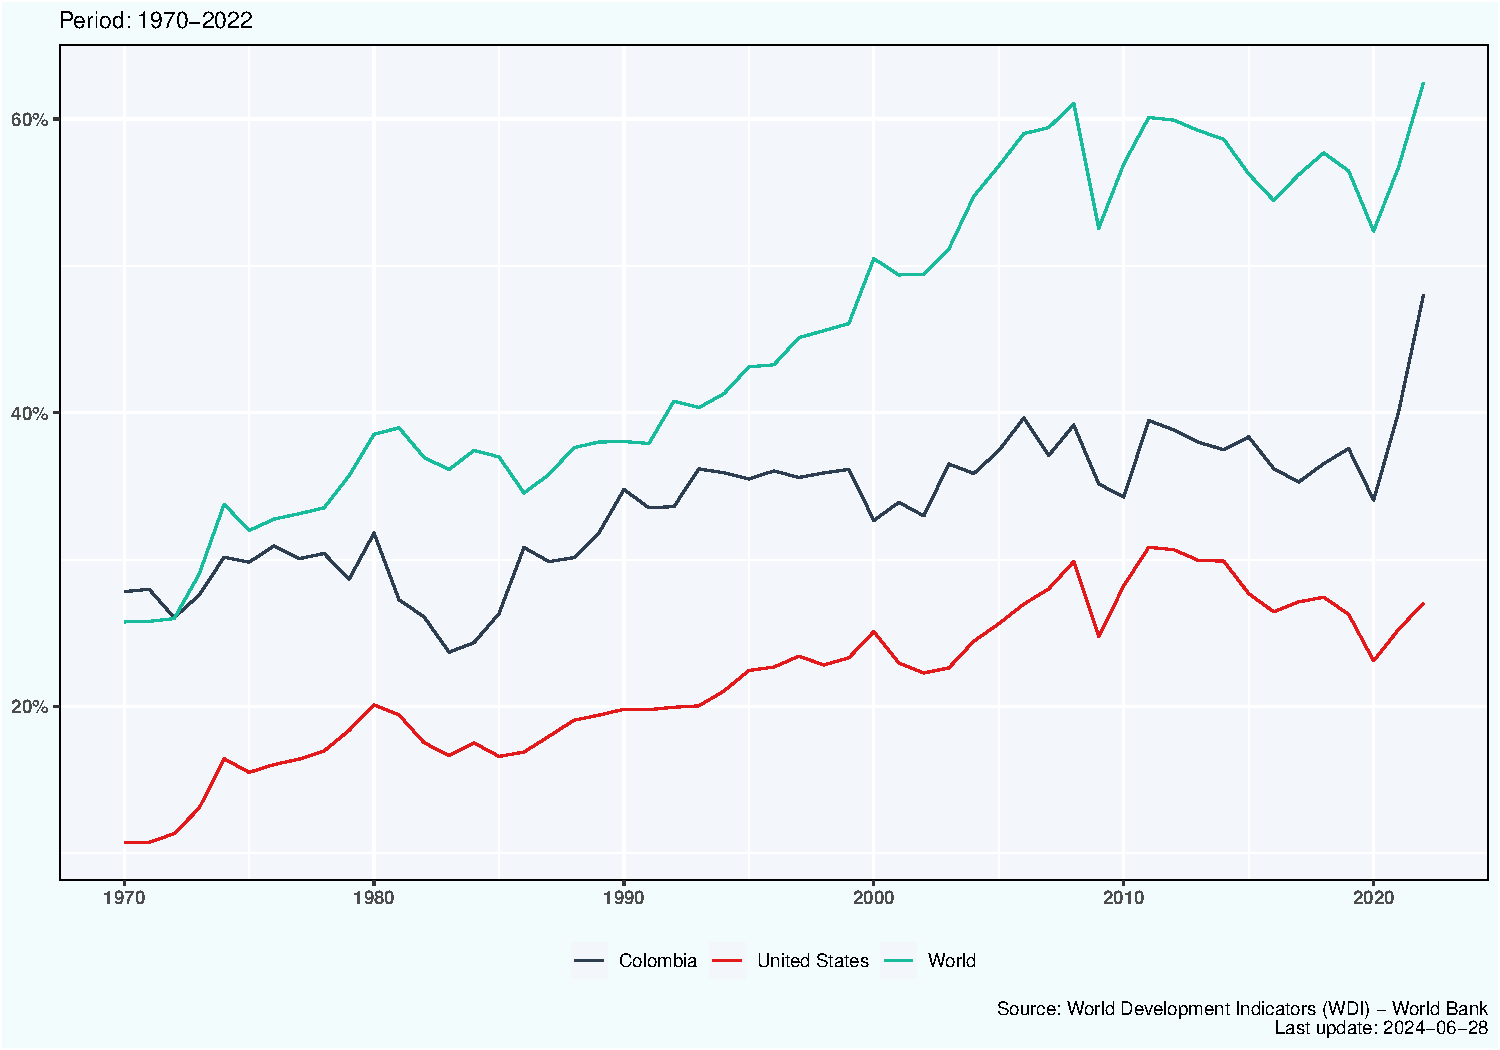
\includegraphics[width=0.85\textwidth,height=\textheight]{005_external_sector_I_files/figure-beamer/fig-trade-col-usa-world-1.pdf}

}

\caption{\label{fig-trade-col-usa-world}Trade (\% of GDP) for Colombia,
USA and the World}

\end{figure}%
\end{frame}

\section{Balance of payments}\label{balance-of-payments}

\begin{frame}{}
\phantomsection\label{section-4}
\begin{itemize}
\item
  The balance of payments is a ``statistical statement that summarizes
  transactions between residents and nonresidents during a period''
  (\citeproc{ref-international_monetary_fund_balance_2009}{Fund 2009,
  para. 2.12})
\item
  It consist of the following accounts:

  \begin{itemize}
  \item
    \textbf{Current account}

    \begin{itemize}
    \tightlist
    \item
      Goods and services account
    \item
      Primary income account
    \item
      Secondary income account
    \end{itemize}
  \item
    \textbf{Capital account}
  \item
    \textbf{Financial account}
  \end{itemize}
\item
  In the case of Colombia you can find the balance of payments in

  \begin{itemize}
  \tightlist
  \item
    \url{https://www.banrep.gov.co/} \textgreater{} Estadísticas
    económicas \textgreater{} Sector externo, tasas de cambio y
    derivados \textgreater{} 1. Sector Externo \textgreater{} Balanza de
    pagos (estadísticas económicas)
  \end{itemize}
\end{itemize}
\end{frame}

\begin{frame}{}
\phantomsection\label{section-5}
\begin{itemize}
\item
  \textbf{Current account}: ``shows flows of goods, services, primary
  income, and secondary income between residents and nonresidents''
  (\citeproc{ref-international_monetary_fund_balance_2009}{Fund 2009,
  para. 2.14})

  \begin{itemize}
  \item
    \textbf{Goods and services account}: ``shows transactions in items
    that are outcomes of production activities''
    (\citeproc{ref-international_monetary_fund_balance_2009}{Fund 2009,
    para. 10.1})
  \item
    \textbf{Primary income account}: ``captures returns for the
    provision of labor and financial assets and renting of natural
    resources''
    (\citeproc{ref-international_monetary_fund_balance_2009}{Fund 2009,
    para. 11.5}) between resident and nonresident institutional units
  \item
    \textbf{Secondary income account}: shows current transfers between
    residents and nonresidents
    (\citeproc{ref-international_monetary_fund_balance_2009}{Fund 2009,
    para. 12.1})
  \end{itemize}
\end{itemize}
\end{frame}

\begin{frame}{}
\phantomsection\label{section-6}
\begin{table}

\caption{\label{tbl-annual-summary-balance-of-payments-current-account-col}Balance
of payments current account Colombia (Annual summary)}

\centering{

\centering\begingroup\fontsize{6}{8}\selectfont

\begin{threeparttable}
\begin{tabular}{lrrr}
\toprule
Account & 2021\textsuperscript{a} & 2022\textsuperscript{b} & 2023\textsuperscript{b}\\
\midrule
\cellcolor[HTML]{e31a1c}{\textbf{1 Cuenta corriente}} & \cellcolor[HTML]{e31a1c}{\textbf{-17949}} & \cellcolor[HTML]{e31a1c}{\textbf{-21205}} & \cellcolor[HTML]{e31a1c}{\textbf{-9154}}\\
    Crédito (exportaciones) & 68783 & 93943 & 91476\\
    Débito (importaciones) & 86732 & 115148 & 100629\\
\cellcolor[HTML]{18BC9C}{\textbf{      1.A Bienes y servicios}} & \cellcolor[HTML]{18BC9C}{\textbf{-20001}} & \cellcolor[HTML]{18BC9C}{\textbf{-16427}} & \cellcolor[HTML]{18BC9C}{\textbf{-7989}}\\
         Crédito (exportaciones) & 50913 & 73287 & 68286\\
         Débito (importaciones) & 70914 & 89714 & 76275\\
\cellcolor[HTML]{CCBE93}{           1.A.a Bienes} & \cellcolor[HTML]{CCBE93}{-13984} & \cellcolor[HTML]{CCBE93}{-12178} & \cellcolor[HTML]{CCBE93}{-6732}\\
              Crédito (exportaciones) & 42736 & 59473 & 52642\\
              Débito (importaciones) & 56719 & 71652 & 59373\\
\cellcolor[HTML]{CCBE93}{\hspace{3.5em}1.A.b Servicios} & \cellcolor[HTML]{CCBE93}{-6017} & \cellcolor[HTML]{CCBE93}{-4249} & \cellcolor[HTML]{CCBE93}{-1258}\\
              Crédito (exportaciones) & 8178 & 13813 & 15644\\
              Débito (importaciones) & 14195 & 18062 & 16902\\
\cellcolor[HTML]{18BC9C}{\textbf{      1.B Ingreso primario (Renta factorial)}} & \cellcolor[HTML]{18BC9C}{\textbf{-8723}} & \cellcolor[HTML]{18BC9C}{\textbf{-17086}} & \cellcolor[HTML]{18BC9C}{\textbf{-14100}}\\
         Crédito & 5932 & 6975 & 8777\\
         Débito & 14656 & 24061 & 22877\\
\cellcolor[HTML]{18BC9C}{\textbf{      1.C Ingreso secundario (Transferencias corrientes)}} & \cellcolor[HTML]{18BC9C}{\textbf{10775}} & \cellcolor[HTML]{18BC9C}{\textbf{12308}} & \cellcolor[HTML]{18BC9C}{\textbf{12936}}\\
         Crédito & 11937 & 13681 & 14413\\
         Débito & 1162 & 1373 & 1477\\
\bottomrule
\end{tabular}
\begin{tablenotes}
\item Source: Banco de la República - Colombia
\item Last update: 2024-07-16
\item[1] Methodology: Sixth version of the Balance of Payments Manual
\item[a] Revised data (Millions of current USD)
\item[b] Provisional data (Millions of current USD)
\end{tablenotes}
\end{threeparttable}
\endgroup{}

}

\end{table}%
\end{frame}

\begin{frame}{}
\phantomsection\label{section-7}
\begin{figure}

\centering{

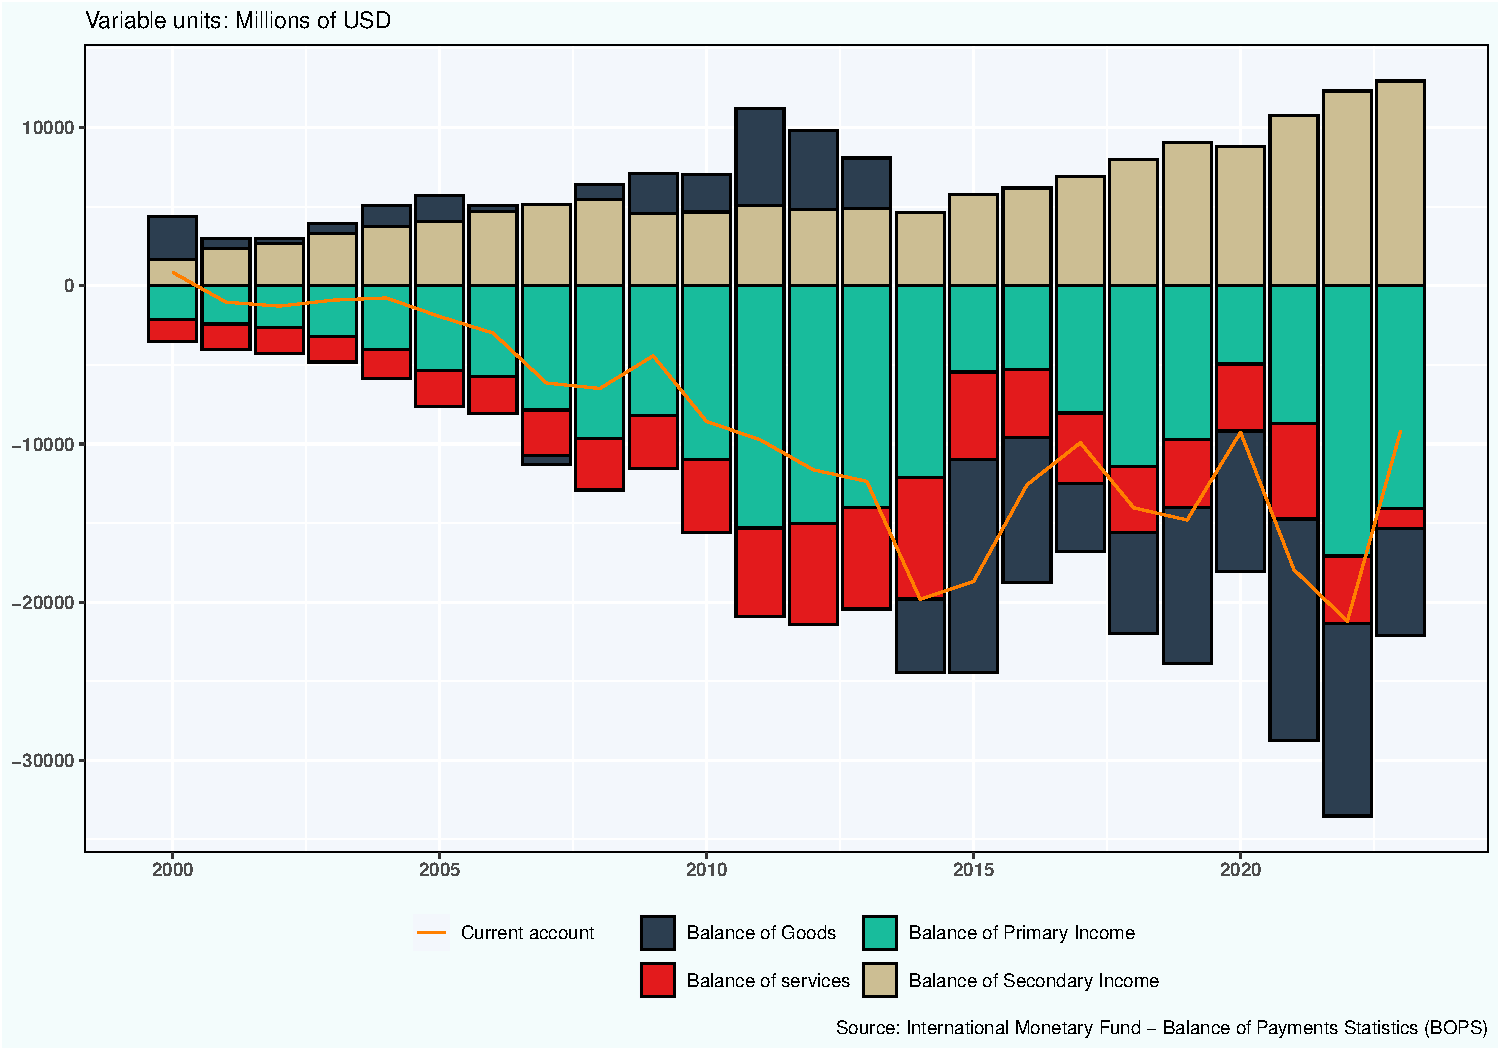
\includegraphics[width=0.85\textwidth,height=\textheight]{005_external_sector_I_files/figure-beamer/fig-current-account-components-col-1.pdf}

}

\caption{\label{fig-current-account-components-col}Current account and
its components for Colombia}

\end{figure}%
\end{frame}

\begin{frame}{}
\phantomsection\label{section-8}
\begin{itemize}
\item
  \textbf{Capital account}

  \begin{itemize}
  \item
    The capital account shows credit and debit entries for nonproduced
    nonfinancial assets and capital transfers between residents and
    nonresidents
    (\citeproc{ref-international_monetary_fund_balance_2009}{Fund 2009,
    para. 2.16})
  \item
    The Capital account does not appear in the balance of payments of
    Colombia because the sources of information currently available do
    not allow the identification and registration of capital transfers
  \end{itemize}
\end{itemize}
\end{frame}

\begin{frame}{}
\phantomsection\label{section-9}
\begin{itemize}
\item
  \textbf{Financial account}: The financial account records transactions
  that involve financial assets and liabilities and that take place
  between residents and nonresidents
  (\citeproc{ref-international_monetary_fund_balance_2009}{Fund 2009,
  para. 8.1})

  \begin{itemize}
  \tightlist
  \item
    \textbf{Direct Investment}: ``is a category of cross-border
    investment associated with a resident in one economy having control
    or a significant degree of influence on the management of an
    enterprise that is resident in another economy''
    (\citeproc{ref-international_monetary_fund_balance_2009}{Fund 2009,
    para. 6.8})
  \item
    \textbf{Portfolio investment}: ``is defined as cross-border
    transactions and positions involving debt or equity securities,
    other than those included in direct investment or reserve assets''
    (\citeproc{ref-international_monetary_fund_balance_2009}{Fund 2009,
    para. 6.54})
  \end{itemize}
\end{itemize}
\end{frame}

\begin{frame}{}
\phantomsection\label{section-10}
\begin{itemize}
\item
  \textbf{Financial account}: ``records transactions that involve
  financial assets and liabilities and that take place between residents
  and nonresidents''
  (\citeproc{ref-international_monetary_fund_balance_2009}{Fund 2009,
  para. 8.1})

  \begin{itemize}
  \item
    \textbf{Financial Derivatives (Other Than Reserves) and Employee
    Stock Options}:

    \begin{itemize}
    \item
      ``A financial derivative contract is a financial instrument that
      is linked to another specific financial instrument or indicator or
      commodity and through which specific financial risks'' \ldots{}
      ``can be traded in their own right in financial markets''
      (\citeproc{ref-international_monetary_fund_balance_2009}{Fund
      2009, para. 5.80})
    \item
      ``Employee stock options are options to buy the equity of a
      company, offered to employees of the company as a form of
      remuneration''
      (\citeproc{ref-international_monetary_fund_balance_2009}{Fund
      2009, para. 5.96})
    \end{itemize}
  \end{itemize}
\end{itemize}
\end{frame}

\begin{frame}{}
\phantomsection\label{section-11}
\begin{itemize}
\item
  \textbf{Financial account}: ``records transactions that involve
  financial assets and liabilities and that take place between residents
  and nonresidents''
  (\citeproc{ref-international_monetary_fund_balance_2009}{Fund 2009,
  para. 8.1})

  \begin{itemize}
  \tightlist
  \item
    \textbf{Other Investment}
    (\citeproc{ref-international_monetary_fund_balance_2009}{Fund 2009,
    paras. 8.42--8.54})
  \item
    \textbf{Reserve Assets}
    (\citeproc{ref-international_monetary_fund_balance_2009}{Fund 2009,
    paras. 8.55--8.57})
  \end{itemize}
\end{itemize}
\end{frame}

\begin{frame}{}
\phantomsection\label{section-12}
\begin{table}

\caption{\label{tbl-annual-summary-balance-of-payments-financial-account-col}Balance
of payments financial account Colombia (Annual summary)}

\centering{

\centering\begingroup\fontsize{4.7}{6.7}\selectfont

\begin{threeparttable}
\begin{tabular}{lrrr}
\toprule
Account & 2021\textsuperscript{a} & 2022\textsuperscript{b} & 2023\textsuperscript{b}\\
\midrule
\cellcolor[HTML]{e31a1c}{\textbf{3 Cuenta financiera}} & \cellcolor[HTML]{e31a1c}{\textbf{-16693}} & \cellcolor[HTML]{e31a1c}{\textbf{-20466}} & \cellcolor[HTML]{e31a1c}{\textbf{-8285}}\\
\cellcolor[HTML]{18BC9C}{\textbf{      3.1 Inversión directa}} & \cellcolor[HTML]{18BC9C}{\textbf{-6381}} & \cellcolor[HTML]{18BC9C}{\textbf{-13799}} & \cellcolor[HTML]{18BC9C}{\textbf{-15972}}\\
\cellcolor[HTML]{CCBE93}{         Adquisición neta de activos financieros} & \cellcolor[HTML]{CCBE93}{3181} & \cellcolor[HTML]{CCBE93}{3384} & \cellcolor[HTML]{CCBE93}{1175}\\
           3.1.1 Participaciones de capital y participaciones en fondos de inversión & 2924 & 2840 & 1610\\
           3.1.2 Instrumentos de deuda & 257 & 543 & -435\\
\cellcolor[HTML]{CCBE93}{         Pasivos netos incurridos} & \cellcolor[HTML]{CCBE93}{9561} & \cellcolor[HTML]{CCBE93}{17183} & \cellcolor[HTML]{CCBE93}{17147}\\
           3.1.1 Participaciones de capital y participaciones en fondos de inversión & 7076 & 14227 & 14224\\
           3.1.2 Instrumentos de deuda & 2485 & 2955 & 2923\\
\cellcolor[HTML]{18BC9C}{\textbf{      3.2 Inversión de cartera}} & \cellcolor[HTML]{18BC9C}{\textbf{-4595}} & \cellcolor[HTML]{18BC9C}{\textbf{427}} & \cellcolor[HTML]{18BC9C}{\textbf{8723}}\\
\cellcolor[HTML]{CCBE93}{         Adquisición neta de activos financieros} & \cellcolor[HTML]{CCBE93}{3751} & \cellcolor[HTML]{CCBE93}{3307} & \cellcolor[HTML]{CCBE93}{9840}\\
           3.2.1 Participaciones de capital y participaciones en fondos de inversión & 2340 & 1056 & 5169\\
           3.2.2 Títulos de deuda & 1411 & 2251 & 4671\\
\cellcolor[HTML]{CCBE93}{         Pasivos netos incurridos} & \cellcolor[HTML]{CCBE93}{8347} & \cellcolor[HTML]{CCBE93}{2880} & \cellcolor[HTML]{CCBE93}{1117}\\
           3.2.1 Participaciones de capital y participaciones en fondos de inversión & -1189 & -551 & 20\\
           3.2.2 Títulos de deuda & 9536 & 3431 & 1097\\
\cellcolor[HTML]{18BC9C}{\textbf{      3.3 Derivados financieros (distintos de reservas) y opciones de compra de acciones por parte de empleados}} & \cellcolor[HTML]{18BC9C}{\textbf{365}} & \cellcolor[HTML]{18BC9C}{\textbf{823}} & \cellcolor[HTML]{18BC9C}{\textbf{-2575}}\\
\cellcolor[HTML]{CCBE93}{         Adquisición neta de activos financieros} & \cellcolor[HTML]{CCBE93}{-419} & \cellcolor[HTML]{CCBE93}{-481} & \cellcolor[HTML]{CCBE93}{-2575}\\
\cellcolor[HTML]{CCBE93}{         Pasivos netos incurridos} & \cellcolor[HTML]{CCBE93}{-784} & \cellcolor[HTML]{CCBE93}{-1305} & \cellcolor[HTML]{CCBE93}{0}\\
\hspace{3em}\cellcolor[HTML]{18BC9C}{\textbf{3.4 Otra inversión}} & \cellcolor[HTML]{18BC9C}{\textbf{-6736}} & \cellcolor[HTML]{18BC9C}{\textbf{-8488}} & \cellcolor[HTML]{18BC9C}{\textbf{-180}}\\
\cellcolor[HTML]{CCBE93}{         Adquisición neta de activos financieros} & \cellcolor[HTML]{CCBE93}{2771} & \cellcolor[HTML]{CCBE93}{4084} & \cellcolor[HTML]{CCBE93}{4003}\\
\cellcolor[HTML]{CCBE93}{         Pasivos netos incurridos} & \cellcolor[HTML]{CCBE93}{9507} & \cellcolor[HTML]{CCBE93}{12573} & \cellcolor[HTML]{CCBE93}{4183}\\
\hspace{3em}\cellcolor[HTML]{18BC9C}{\textbf{3.5 Activos de reserva}} & \cellcolor[HTML]{18BC9C}{\textbf{654}} & \cellcolor[HTML]{18BC9C}{\textbf{571}} & \cellcolor[HTML]{18BC9C}{\textbf{1718}}\\
\cellcolor[HTML]{e31a1c}{\textbf{Errores y omisiones netos}} & \cellcolor[HTML]{e31a1c}{\textbf{1256}} & \cellcolor[HTML]{e31a1c}{\textbf{739}} & \cellcolor[HTML]{e31a1c}{\textbf{868}}\\
\bottomrule
\end{tabular}
\begin{tablenotes}
\item Source: Banco de la República - Colombia
\item Last update: 2024-07-16
\item[1] Methodology: Sixth version of the Balance of Payments Manual
\item[a] Revised data (Millions of current USD)
\item[b] Provisional data (Millions of current USD)
\end{tablenotes}
\end{threeparttable}
\endgroup{}

}

\end{table}%
\end{frame}

\begin{frame}{}
\phantomsection\label{section-13}
\begin{figure}

\centering{

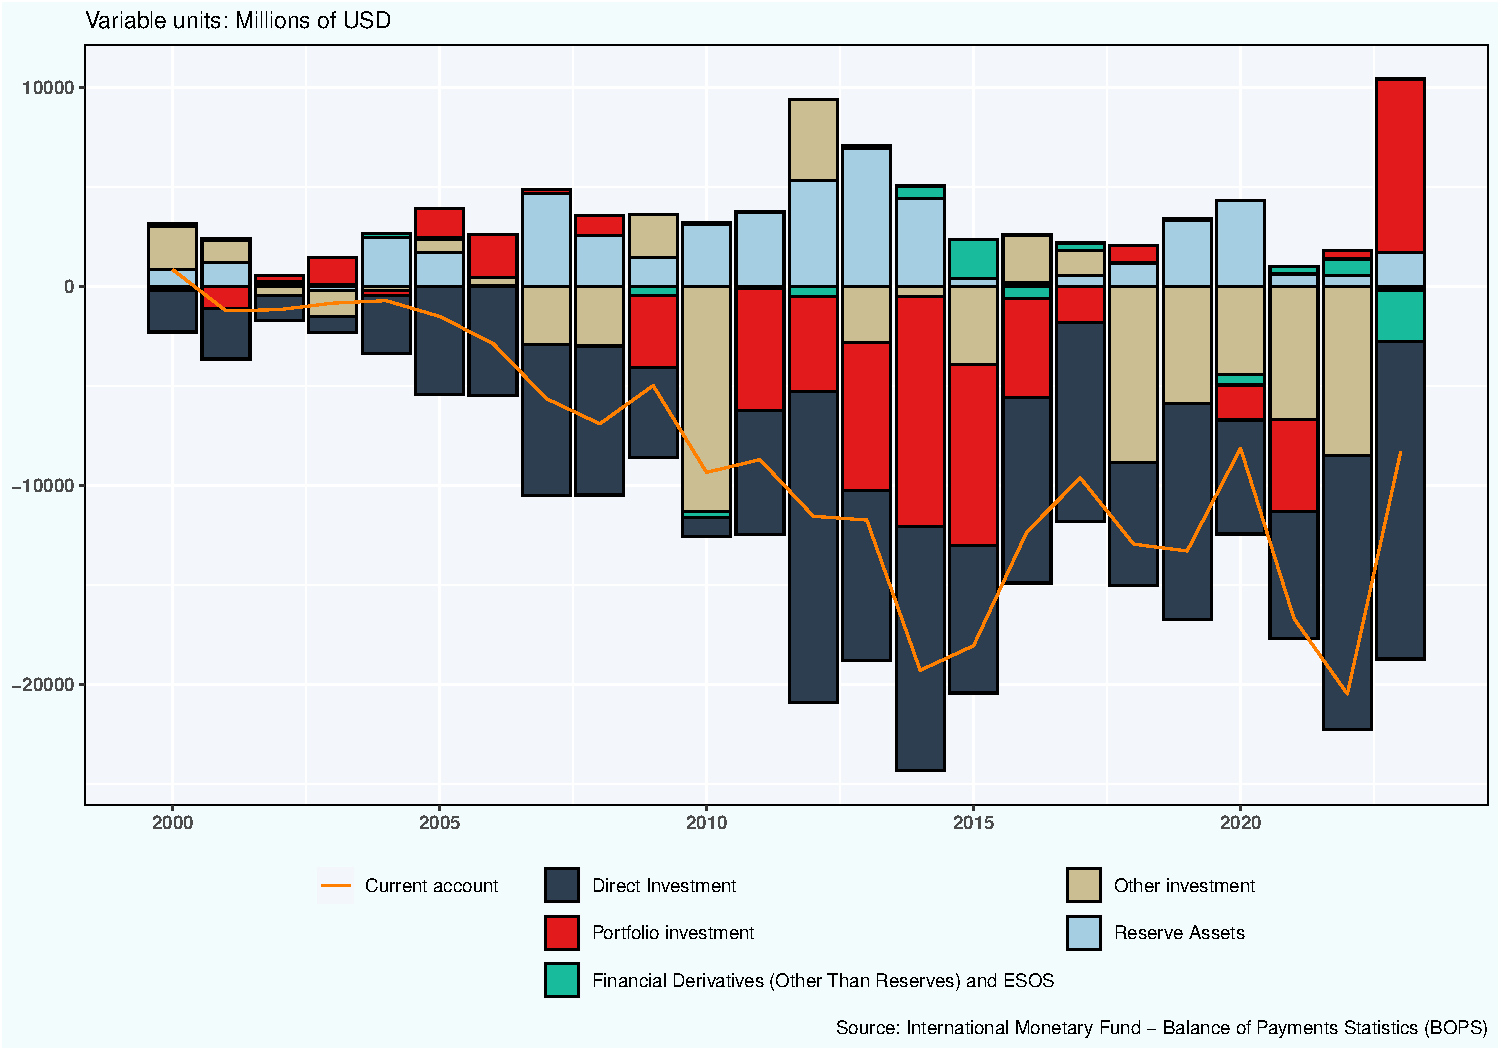
\includegraphics[width=0.85\textwidth,height=\textheight]{005_external_sector_I_files/figure-beamer/fig-financial-account-components-col-1.pdf}

}

\caption{\label{fig-financial-account-components-col}Financial account
and its components for Colombia}

\end{figure}%
\end{frame}

\begin{frame}{}
\phantomsection\label{section-14}
\begin{itemize}
\item
  \textbf{Net errors and omissions}

  \begin{itemize}
  \tightlist
  \item
    Financial account - (Current account + Capital account) = Net errors
    and omissions
  \end{itemize}
\end{itemize}
\end{frame}

\begin{frame}{}
\phantomsection\label{section-15}
\begin{figure}

\centering{

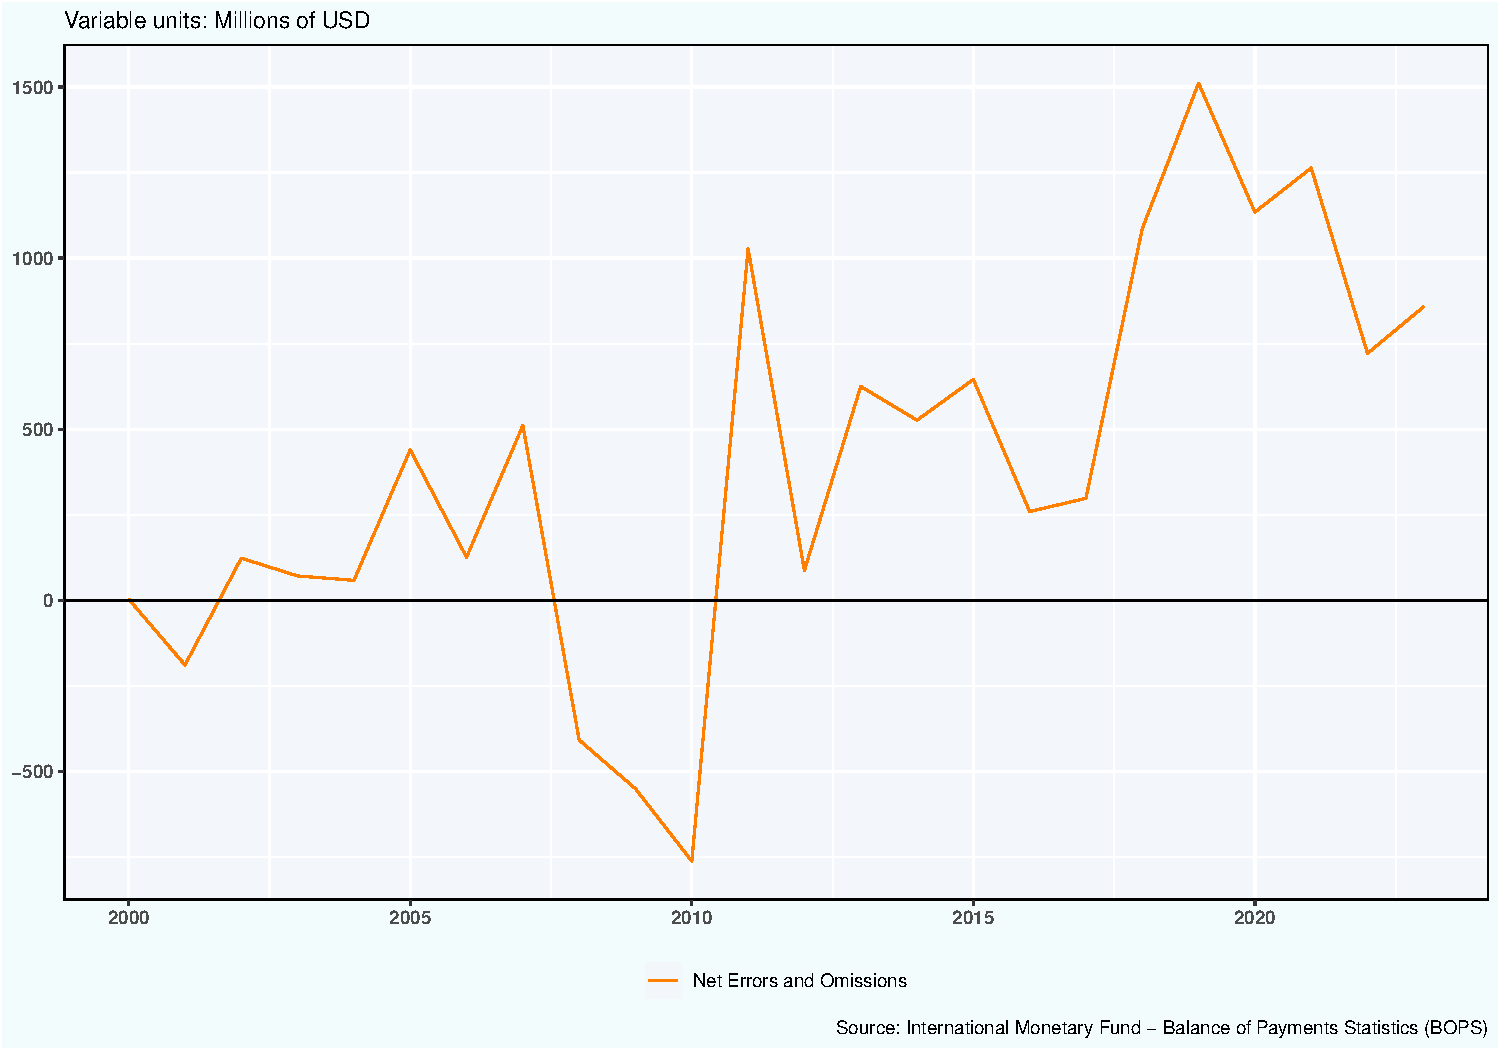
\includegraphics[width=0.85\textwidth,height=\textheight]{005_external_sector_I_files/figure-beamer/fig-net-errors-omissions-col-1.pdf}

}

\caption{\label{fig-net-errors-omissions-col}Net Errors and Omissions
for Colombia}

\end{figure}%
\end{frame}

\begin{frame}{}
\phantomsection\label{section-16}
\begin{itemize}
\item
  \textbf{Accounting Framework}

  \begin{itemize}
  \item
    \textbf{Double-entry bookkeeping}

    \begin{itemize}
    \tightlist
    \item
      For every transaction between an Colombia resident and the rest of
      the world, the balance of payments will record two entries
      (\citeproc{ref-rba_balance_2021}{RBA 2021})
    \end{itemize}
  \item
    \textbf{Credits} \((+)\)

    \begin{itemize}
    \tightlist
    \item
      Outflows of real resources (exports)
    \item
      Decrease in financial assest
    \item
      Increase in liabilities
    \end{itemize}
  \item
    \textbf{Debits} \((-)\)

    \begin{itemize}
    \tightlist
    \item
      Inflows of real resources (imports)
    \item
      Increase in financial assest
    \item
      Decrease in liabilities
    \end{itemize}
  \end{itemize}
\end{itemize}
\end{frame}

\begin{frame}{}
\phantomsection\label{section-17}
\begin{itemize}
\item
  Examples taken from (\citeproc{ref-rba_balance_2021}{RBA 2021}) and
  adapted for Colombia

  \begin{enumerate}
  \item
    A Colombian mining company exports \$100 million of iron ore to a
    private Chinese steel maker
  \item
    Colombian residents go on overseas to Panama and spend a total of
    \$5 million. The Colombian residents pay by using money deposited in
    their Colombian bank accounts
  \item
    Colombian resident, buys \$20 million of shares in a company listed
    on the New York Stock Exchange, equivalent to less than 10 per cent
    of the voting rights in that company. The shares are paid for using
    money from the resident's bank account in Colombia
  \end{enumerate}
\end{itemize}
\end{frame}

\begin{frame}{}
\phantomsection\label{section-18}
\begin{table}

\caption{\label{tbl-sample-balance-of-payments}Sample of Balance of
Payments}

\centering{

\centering\begingroup\fontsize{12}{14}\selectfont

\begin{threeparttable}
\begin{tabular}{llll}
\toprule
\textbf{Account} & \textbf{Credit} & \textbf{Debit} & \textbf{Net}\\
\midrule
\textbf{Current account} & \textbf{100} & \textbf{-5} & \textbf{95}\\
\hspace{1em}Trade balance & 100 & -5 & 95\\
\hspace{2em}Goods & 100¹ &  & 100\\
\hspace{2em}Services &  & -5² & -5\\
\textbf{Financial account} & \textbf{25} & \textbf{-120} & \textbf{-95}\\
\hspace{1em}Portfolio investment &  & -20³ & -20\\
\hspace{1em}Other investment & 5² & -100¹ & -75\\
 & 20³ &  & \\
\textbf{Balance of payments} & \textbf{125} & \textbf{-125} & \textbf{0}\\
\bottomrule
\end{tabular}
\begin{tablenotes}
\item *The superscripts indicate the examples' transactions
\end{tablenotes}
\end{threeparttable}
\endgroup{}

}

\end{table}%
\end{frame}

\section{Acknowledgments}\label{acknowledgments}

\begin{frame}{}
\phantomsection\label{section-19}
\begin{itemize}
\item
  To my family that supports me
\item
  To the taxpayers of Colombia and the
  \href{https://www.umng.edu.co/estudiante}{\textbf{UMNG students}} who
  pay my salary
\item
  To the \href{https://www.business-science.io/}{\textbf{Business
  Science}} and \href{https://www.rfordatasci.com/}{\textbf{R4DS Online
  Learning}} communities where I learn
  \href{https://www.r-project.org/about.html}{\textbf{R}} and
  \href{https://www.python.org/about/}{\textbf{\(\pi\)-thon}}
\item
  To the \href{https://www.r-project.org/contributors.html}{\textbf{R
  Core Team}}, the creators of
  \href{https://rstudio.com/products/rstudio/}{\textbf{RStudio IDE}},
  \href{https://quarto.org/}{\textbf{Quarto}} and the authors and
  maintainers of the packages
  \href{https://CRAN.R-project.org/package=tidyverse}{\textbf{tidyverse}},
  \href{https://CRAN.R-project.org/package=wbstats}{\textbf{wbstats}},
  \href{https://CRAN.R-project.org/package=tidyquant}{\textbf{tidyquant}},
  \href{https://CRAN.R-project.org/package=readxl}{\textbf{readxl}},
  \href{https://CRAN.R-project.org/package=knitr}{\textbf{knitr}},
  \href{https://CRAN.R-project.org/package=kableExtra}{\textbf{kableExtra}},
  \href{https://CRAN.R-project.org/package=imfr}{\textbf{imfr}}, and
  \href{https://CRAN.R-project.org/package=tinytex}{\textbf{tinytex}}
  for allowing me to access these tools without paying for a license
\item
  To the \href{https://www.kernel.org/category/about.html}{\textbf{Linux
  kernel community}} for allowing me the possibility to use some
  \href{https://static.lwn.net/Distributions/}{\textbf{Linux
  distributions}} as my main
  \href{https://en.wikipedia.org/wiki/Operating_system}{\textbf{OS}}
  without paying for a license
\end{itemize}
\end{frame}

\section*{References}\label{references}
\addcontentsline{toc}{section}{References}

\begin{frame}[allowframebreaks]{References}
\phantomsection\label{refs}
\begin{CSLReferences}{1}{0}
\bibitem[\citeproctext]{ref-cardenas_introduccion_2020}
Cardenas, Mauricio. 2020. \emph{Introducción a La {Economía}
{Colombiana}}. 4th ed. Alfaomega.

\bibitem[\citeproctext]{ref-international_monetary_fund_balance_2009}
Fund, International Monetary, ed. 2009. \emph{Balance of Payments and
International Investment Position Manual}. 6th ed. Washington D.C:
International Monetary Fund.

\bibitem[\citeproctext]{ref-rba_balance_2021}
RBA. 2021. {``The {Balance} of {Payments} {\textbar} {Explainer}
{\textbar} {Education}.''} \emph{Reserve Bank of Australia}.
\url{https://www.rba.gov.au/education/resources/explainers/the-balance-of-payments.html}.

\end{CSLReferences}
\end{frame}




\end{document}
